\documentclass[a4paper]{article}
\usepackage[a4paper,margin=0mm]{geometry}
\usepackage{fontspec}
\usepackage{unicode-math}
\usepackage{tikz}
\usetikzlibrary{fit,calc,positioning,arrows.meta}
\usepackage[table]{xcolor}
\usepackage[absolute]{textpos}
\usepackage{array}

\setmainfont{Libertinus Serif}
\setsansfont{Libertinus Sans}
\setmathfont{Libertinus Math}

\definecolor{accent}{HTML}{602785}
\definecolor{badge}{HTML}{B8A0C8}
\definecolor{ink}{HTML}{2A2E30}

\setlength{\TPHorizModule}{1mm}
\setlength{\TPVertModule}{1mm}
\setlength{\parindent}{0pt}
\pagestyle{empty}

\newcommand{\topicheader}[2]{%
\begin{textblock*}{194mm}(16mm,10mm)
\begin{tikzpicture}
\node[fill=accent,text=white,font=\sffamily\bfseries\fontsize{13}{13}\selectfont,
      minimum width=9mm,minimum height=9mm,inner sep=0pt] at (4.5mm,-4.5mm) {#1};
\node[font=\sffamily\bfseries\fontsize{15}{16}\selectfont,text=ink,anchor=west] at (12mm,-4.5mm) {#2};
\end{tikzpicture}
\end{textblock*}
\begin{textblock*}{194mm}(16mm,22.5mm)

\begin{tikzpicture}
\fill[accent] (0,0) rectangle (194mm,0.5mm);
\end{tikzpicture}
\end{textblock*}
}

\newcommand{\pagekicker}[1]{%
\begin{textblock*}{100mm}(16mm,25.5mm)
\begin{tikzpicture}
\node[fill=ink,text=white,font=\sffamily\bfseries\fontsize{8}{8}\selectfont,
      inner sep=2.2pt,rounded corners=1pt] {\MakeUppercase{#1}};
\end{tikzpicture}
\end{textblock*}
}

\newcommand{\videobanner}[1]{%
\begin{textblock*}{178mm}(16mm,25.5mm)
\begin{tikzpicture}
\fill[accent] (0,0) rectangle (178mm,-10mm);
\draw[white,line width=0.6pt] (3mm,-1.7mm) rectangle (11.5mm,-8.3mm);
\node[white,font=\sffamily\fontsize{4}{4.4}\selectfont,align=center] at (7.25mm,-5mm) {QR\\CODE};
\node[white,font=\sffamily\bfseries\fontsize{9.5}{11}\selectfont,anchor=west] at (16mm,-5.6mm) {WATCH THE VIDEO BEFORE YOU SOLVE};
\node[white,font=\sffamily\fontsize{7.5}{8}\selectfont,anchor=east] at (174mm,-5.6mm) {YouTube ~\textbullet~ #1};
\end{tikzpicture}
\end{textblock*}
}

\newcommand{\pagefooter}[1]{%
\begin{textblock*}{194mm}(8mm,286.41mm)
  
\begin{tikzpicture}
    \fill[accent] (0,0) rectangle (194mm,0.6mm);
  \end{tikzpicture}
\end{textblock*}
\begin{textblock*}{63.59mm}(8mm,288.27mm)
  {\sffamily\bfseries\color{accent}\fontsize{13}{16}\selectfont SAT 1200+}
\end{textblock*}
\begin{textblock*}{10mm}(188mm,288.27mm)
  \centering{\sffamily\color{accent}\fontsize{14}{16}\selectfont #1}
\end{textblock*}
}

\newcommand{\cardbg}[4]{%
\begin{textblock*}{#3mm}(#1mm,#2mm)
\begin{tikzpicture}
\fill[badge!22,rounded corners=3mm] (0,0) rectangle (#3mm,-#4mm);
\end{tikzpicture}
\end{textblock*}%
}

\newcommand{\pill}[3]{%
\begin{textblock*}{160mm}(#1mm,#2mm)
\begin{tikzpicture}
\node[fill=accent,text=white,anchor=north west,font=\sffamily\bfseries\fontsize{10}{10}\selectfont,
      rounded corners=8pt,inner xsep=5mm,inner ysep=1.8mm] at (0,0) {RULE ~\textperiodcentered~ #3};
\end{tikzpicture}
\end{textblock*}%
}

\arrayrulecolor{accent}
\setlength{\arrayrulewidth}{0.7pt}
\renewcommand{\arraystretch}{1.5}

\begin{document}

% ======================================================================
% PAGE 1
% ======================================================================
\topicheader{22}{Right-Triangle Trigonometry}
\videobanner{Lesson 22}
\pagefooter{118}
\mbox{}%

% ---- CARD 1: SOH-CAH-TOA ----
\cardbg{16}{40}{178}{92}
\pill{26}{43}{Right-triangle ratios (SOH-CAH-TOA)}

\begin{textblock*}{85mm}(26mm,58mm)
{\fontsize{13}{22}\selectfont
$\sin\theta=\dfrac{\text{opp}}{\text{hyp}}\quad
\cos\theta=\dfrac{\text{adj}}{\text{hyp}}\quad
\tan\theta=\dfrac{\text{opp}}{\text{adj}}$}
\end{textblock*}

\begin{textblock*}{70mm}(120mm,60mm)
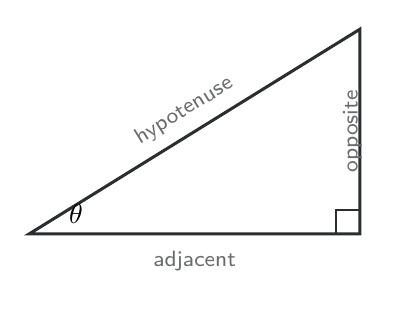
\begin{tikzpicture}
\draw[ink,line width=1.1pt] (0,0) -- (42mm,0) -- (42mm,26mm) -- cycle;
\draw[ink,line width=0.8pt] (39mm,0) -- (39mm,3mm) -- (42mm,3mm);
\node[font=\fontsize{10}{10}\selectfont] at (6mm,2.5mm) {$\theta$};
\node[font=\sffamily\fontsize{8}{8}\selectfont,text=ink!70,below] at (21mm,-1mm) {adjacent};
\node[font=\sffamily\fontsize{8}{8}\selectfont,text=ink!70,rotate=90,anchor=south] at (43.5mm,13mm) {opposite};
\node[font=\sffamily\fontsize{8}{8}\selectfont,text=ink!70,rotate=31.7,anchor=south] at (21mm,13.5mm) {hypotenuse};
\end{tikzpicture}
\end{textblock*}

\begin{textblock*}{158mm}(26mm,102mm)
{\fontsize{10.5}{13}\selectfont\color{ink}
\textbf{SOH-CAH-TOA:} Sin = Opp/Hyp, Cos = Adj/Hyp, Tan = Opp/Adj. Ratios are
unitless.}
\end{textblock*}

% ---- CARD 2: opposite/adjacent depend on the angle ----
\cardbg{16}{138}{178}{90}
\pill{26}{141}{Opposite \& adjacent flip with the angle}

\begin{textblock*}{158mm}(26mm,154mm)
{\fontsize{10.5}{13}\selectfont\color{ink}
The same leg is opposite for one acute angle and adjacent for the other --
redefine them each time the angle changes.}
\end{textblock*}

\begin{textblock*}{158mm}(26mm,167mm)
{\fontsize{10.5}{13}\selectfont
3-4-5 triangle, legs $BC=3$, $AC=4$, hyp $AB=5$:\\[2mm]
\begin{tabular}{|p{40mm}|>{\centering\arraybackslash}p{30mm}|>{\centering\arraybackslash}p{30mm}|}
\hline
\rowcolor{accent}
{\color{white}} & {\color{white}\textbf{From $A$}} & {\color{white}\textbf{From $B$}} \\ \hline
opposite & $3$ & $4$ \\ \hline
adjacent & $4$ & $3$ \\ \hline
\end{tabular}}
\end{textblock*}

\clearpage

% ======================================================================
% PAGE 2
% ======================================================================
\topicheader{22}{Right-Triangle Trigonometry}
\pagekicker{Rules sheet -- 2/2}
\pagefooter{119}
\mbox{}%

% ---- CARD 3: solving for a missing side ----
\cardbg{16}{33}{178}{85}
\pill{26}{36}{Solving for a missing side}

\begin{textblock*}{158mm}(26mm,49mm)
{\fontsize{10.5}{13}\selectfont
\begin{tabular}{|p{65mm}|>{\centering\arraybackslash}p{80mm}|}
\hline
\rowcolor{accent}
{\color{white}\textbf{Known + unknown}} & {\color{white}\textbf{Use}} \\ \hline
hypotenuse + opposite & $\sin$ \\ \hline
hypotenuse + adjacent & $\cos$ \\ \hline
adjacent + opposite & $\tan$ \\ \hline
\end{tabular}}
\end{textblock*}

\begin{textblock*}{158mm}(26mm,90mm)
{\fontsize{11}{14}\selectfont
Hyp $=12$, angle $=25°$, find opposite: $\sin25°=\dfrac{\text{opp}}{12}
\Longrightarrow \text{opp}=12\sin25°\approx5.07$}
\end{textblock*}

\begin{textblock*}{158mm}(26mm,108mm)
{\fontsize{10}{13}\selectfont\color{black!55}\itshape
Keep the calculator in degree mode -- radian mode gives a plausible-looking
but wrong answer with no warning.}
\end{textblock*}

% ---- CARD 4: missing angle + complementary identity ----
\cardbg{16}{125}{178}{90}
\pill{26}{128}{Missing angle \& complementary identity}

\begin{textblock*}{158mm}(26mm,141mm)
{\fontsize{13}{16}\selectfont $\sin\theta=\cos(90°-\theta)$}
\end{textblock*}

\begin{textblock*}{158mm}(26mm,155mm)
{\fontsize{10.5}{13}\selectfont\color{ink}
To find the angle itself, apply the inverse function to the ratio -- the
ratio is not the angle.}
\end{textblock*}

\begin{textblock*}{158mm}(26mm,168mm)
{\fontsize{11}{14}\selectfont
$\sin\theta=\dfrac{7}{25}=0.28\ \Longrightarrow\
\theta=\arcsin(0.28)\approx16.3°$}
\end{textblock*}

\begin{textblock*}{158mm}(26mm,183mm)
{\fontsize{10}{13}\selectfont\color{black!55}\itshape
$\sin\theta=0.6$ means $\theta=\arcsin(0.6)\approx36.9°$ -- not $0.6°$.}
\end{textblock*}

\end{document}
